% Figure 12 of scale_lanes_deck: the DECOUPLED tiers (4 engines : 256 workers : 256 microVMs).
% Each episode joins a free worker, the least-loaded engine and any free microVM; nothing is pinned.
% Build: xelatex lanes_fig12_decoupled.tex  (-> .pdf, included by ../scale_lanes_deck.md)
\documentclass[tikz,border=4pt]{standalone}
\usepackage{fontspec}
\setmainfont{DejaVu Sans}
\setmonofont{DejaVu Sans Mono}
\usetikzlibrary{positioning,arrows.meta,fit,backgrounds,calc}
\definecolor{slime}{RGB}{230,230,230}
\definecolor{host}{RGB}{214,216,240}
\definecolor{gpu}{RGB}{255,236,204}
\definecolor{vm}{RGB}{214,238,220}
\definecolor{ink}{RGB}{40,40,90}
\begin{document}
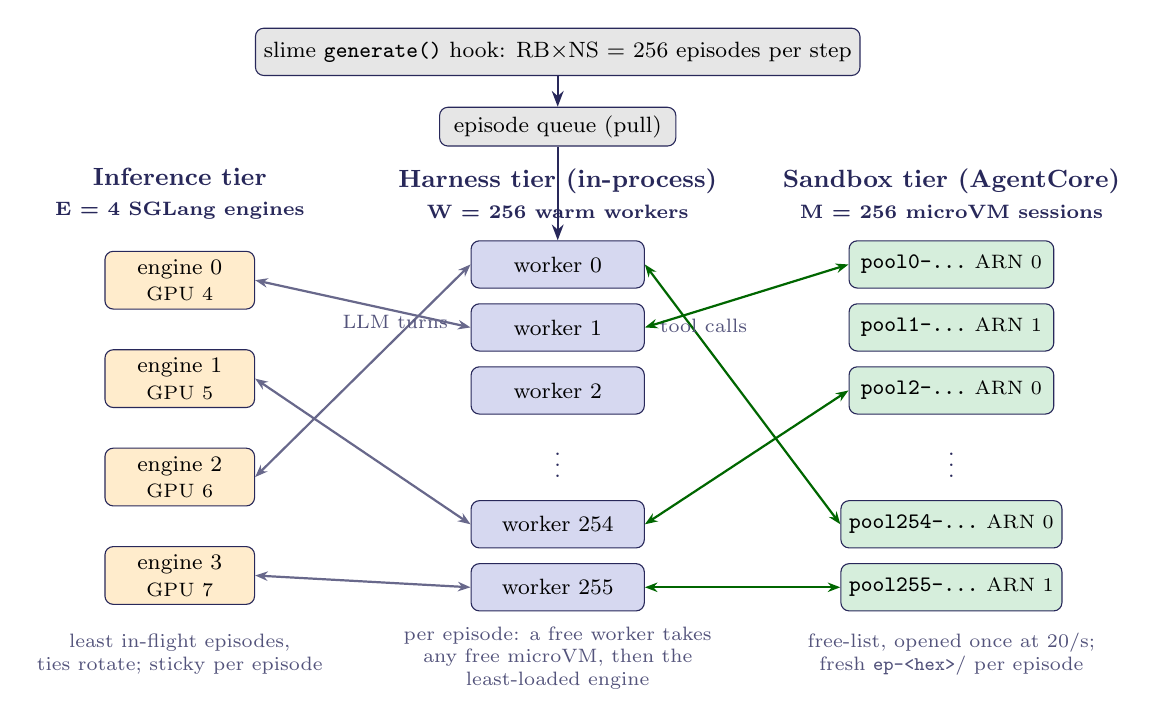
\begin{tikzpicture}[
  font=\footnotesize,
  box/.style={draw=ink, rounded corners=3pt, fill=#1, align=center, inner sep=3pt, minimum height=0.6cm, minimum width=2.2cm},
  line/.style={thick, draw=ink, -{Stealth[length=2mm]}},
  dline/.style={thick, draw=ink!70, {Stealth[length=1.6mm]}-{Stealth[length=1.6mm]}},
  head/.style={font=\small\bfseries, text=ink, align=center},
  note/.style={font=\scriptsize, text=ink!80, align=center},
]
% top: slime feeds one shared episode queue; workers pull from it
\node[box=slime, minimum width=5.2cm] (sl) at (5.2,2.7) {slime \texttt{generate()} hook: RB$\times$NS = 256 episodes per step};
\node[box=slime, minimum width=3.0cm, minimum height=0.45cm] (q) at (5.2,1.75) {episode queue (pull)};
\draw[line] (sl) -- (q);

\node[head] at (0.4,0.9)  {Inference tier\\\scriptsize E = 4 SGLang engines};
\node[head] at (5.2,0.9)  {Harness tier (in-process)\\\scriptsize W = 256 warm workers};
\node[head] at (10.2,0.9) {Sandbox tier (AgentCore)\\\scriptsize M = 256 microVM sessions};

% harness workers
\foreach \w/\n/\y in {0/0/0, 1/1/-0.8, 2/2/-1.6, 3/254/-3.3, 4/255/-4.1} {
  \node[box=host] (h\w) at (5.2,\y) {worker \n};
}
\node[text=ink] at (5.2,-2.45) {$\vdots$};
\draw[line] (q.south) -- (h0.north);

% engines (left)
\foreach \e/\y in {0/-0.2, 1/-1.45, 2/-2.7, 3/-3.95} {
  \node[box=gpu, minimum width=1.9cm] (e\e) at (0.4,\y) {engine \e\\\scriptsize GPU \the\numexpr\e+4\relax};
}
\node[note] at (0.4,-4.95) {least in-flight episodes,\\ties rotate; sticky per episode};

% microVM sessions (right)
\foreach \s/\n/\a/\y in {0/0/0/0, 1/1/1/-0.8, 2/2/0/-1.6, 3/254/0/-3.3, 4/255/1/-4.1} {
  \node[box=vm, minimum width=2.6cm] (v\s) at (10.2,\y) {\texttt{pool\n-…}\ \scriptsize ARN \a};
}
\node[text=ink] at (10.2,-2.45) {$\vdots$};
\node[note] at (10.2,-4.95) {free-list, opened once at 20/s;\\fresh \texttt{ep-<hex>}/ per episode};

% example joins: crossing on purpose (nothing is pinned)
\draw[dline] (h0.west) -- node[above, note, pos=0.35] {LLM turns} (e2.east);
\draw[dline] (h1.west) -- (e0.east);
\draw[dline] (h3.west) -- (e1.east);
\draw[dline] (h4.west) -- (e3.east);
\draw[dline, draw=green!40!black] (h0.east) -- node[above, note, pos=0.3] {tool calls} (v3.west);
\draw[dline, draw=green!40!black] (h1.east) -- (v0.west);
\draw[dline, draw=green!40!black] (h3.east) -- (v2.west);
\draw[dline, draw=green!40!black] (h4.east) -- (v4.west);
\node[note] at (5.2,-5.0) {per episode: a free worker takes\\any free microVM, then the\\least-loaded engine};
\end{tikzpicture}
\end{document}
